%. Pedigrees, allele frequencies, and lineages
% * recombination, segregation, and mutation
% * Moran and Cannings models
%   * including general, nonhomogeneous
%   * as generating a pedigree
% * forwards and reverse processes
% * limiting, continuous process


%%%%%%% %%%%%%%%
\section*{General goal}

Perhaps we are presented with data: genome sequences plus other information
about a number of individuals that are usually random samples from some population(s),
and we want to learn about their shared history: 
estimate levels of relatedness between the samples;
infer their ancestral genome sequence(s);
or identify genomic locations subject to selection.
Or, perhaps we want to compute the levels of genetic diversity 
predicted under a certain population model .
In either case, we must understand the relationship between process parameters
(e.g.\ migration rates, selection coefficients)
and the observed genomic patterns of dissimilarity.

This will start out from the unconvential direction
of treating the usual population genetic quantities as summary statistics
of the (unobserved) pedigree--with--recombination.
Usually, things like ``coalescent time'' are only defined in the context of mathematical models,
but can equally well be thought of as descriptive statistics,
whose expected values we can compute under certain models.
This seems to me at least conceptually useful when thinking about such quantities
as estimated from real data, where assumptions such as random mating are rarely met.


%%%%%%% %%%%%%%%
\section{Recombination, segregation, and mutation}

First, an outline of how we model diploid reproduction, i.e.\ making a new genome out of the genomes of the parents.
There are exceptions (of course), but mostly,
each organism has two copies of each chromosome (counting sex chromosomes as a pair), one from mom and one from dad.
Offspring are the union of two gametes (an egg and a spermatid),
and each gamete is produced by a single diploid cell:
\begin{itemize}
    \item duplicating each chromosome (by mitosis)
    \item recombining the homlogous copies
    \item segregating these copies among four daughter cells.
\end{itemize}
Sometimes all four daughter cells become gametes;
sometimes (e.g.\ female meiosis in mammals) only one will.


\paragraph{Recombination} is complicated, varies along the genome, and is affected by genomic factors and motifs.
To make it tractable, we assume that recombination breakpoints occur as a Poisson point process 
with constant mean of 2 breakpoints per unit of length,
and that each breakpoint is a crossing over between a randomly chosen maternal and a randomly chosen paternal chromosome.
This produces an average of 1 crossover per chromosome per unit length, 
i.e.\ we are measuring length in genetic map length.


\paragraph{Mutation}
Evolution needs ``descent \emph{with modification}'' -- and, from thence comes our data -- so we need mutation, also.
In a major concession to mathematical convenience, we'll simply model mutation as another Poisson point process --
suppose that each gamete differs from its progenitor chromosome at the points of an Poisson point process.
This is the ``infinite sites model'', assuming that mutation cannot hit at the same location twice.
Usually we assume the point process of mutations has mean rate $\mu$ per unit of map length,
but in reality this rate varies along the genome.

\paragraph{Segregation}
Once four gametes are produced, it remains to be decided which of the four produce the offspring.
We assume that one is chosen uniformly at random,
independently of the result of recombination.
(Again, there are exceptions.)


%%%%%%% %%%%%%%%
\section{The pedigree, with recombination}

The \emph{pedigree} of a set of individuals is a graph 
describing all parent-offspring relationships between these
and some set of their ancestors.
The \emph{population pedigree} describes all such relationships
between all individuals living and possibly dead.
This records mate choice,
but omits the important information of recombination and segregation,
i.e.\ which parts of each chromosome derive from which of the parents' two homologous copies.
Adding this information to the pedigree obtains what is known as the \emph{ancestral recombination graph}, or ARG.
There are a number of ways to formalize this notion;
see \citep{marjoram,hudson} for discussions.
One way simply notes that the relatedness structure at any particular locus
is a treelike subset of the pedigree,
and that the collection of these trees -- one for each base in the genome, say --
is sufficient to reconstruct the entire history of inheritance, recombination and segregation.
Alternatively, one can annotate each link in the pedigree with a labeling of the genome by $\{m,p\}$,
denoting which segments of the parent's maternal and paternal chromosomal copies were passed down along that link.
See figure \ref{fig:pedigree_ibd} for a partial depiction.

\begin{figure}[ht!]
  \begin{center}
    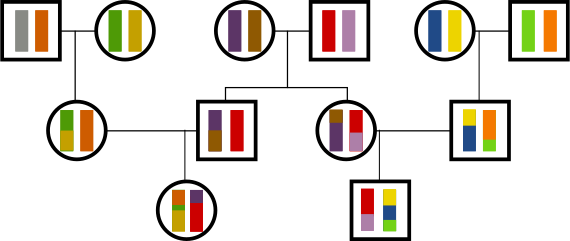
\includegraphics[width=3.5in]{pedigree-ibd-recombination}
  \end{center}
  \caption{
  A small pedigree relating two cousins to their six grandparents,
  with the extra information of recombination and segregation on one chromosome
  encoded by a coloring: each chromosome is composed
  of a patchwork of the grandparental chromosomes.
  \label{fig:pedigree_ibd}
  }
\end{figure}

%%%%%%% %%%%%%%%
\subsection{Coalescence times}

Perhaps the simplest thing we can obtain from the full ancestral recombination graph 
is the typical degree of relatedness of pairs of individuals.
More concretely, we might ask for the empirical distribution
of pairwise times back to the most recent common ancestor
across all pairs of chromosomes and all loci:
the distribution of $\tau_T$, if $\tau_T$ is the length of a randomly chosen one of these paths.

An slightly different way of formulating this is as follows:
pick two random chromosomes and a random locus;
follow the lineages of the two alleles at that locus up through the pedigree
until their common ancestor;
one-half the number of meioses encountered is $\tau_T$.
Since these two lineages will henceforth move together through if followed further back through the pedigree,
$\tau_T$ is known as the ``coalescence time''.

More generally, the phrase ``coalescence time'' is shorthand
for ``number of generations back to the most recent common ancestor'',
taken as a random quantity across random samples of sets of chromosomes and/or loci.
In this formulation, it is the empirical distribution of lengths of a certain set of paths 
to common ancestors through the pedigree.


%%%%%%% %%%%%%%%%%%%
\section{Conventions and definitions}

\paragraph{Generations}
  When two chromosomes share a common ancestor, we like to say that that ancestor lived some number of ``generations'' in the past.
  For most organisms, the notion of a generation is statistical, rather than a fixed quantity.
  What we actually care about is the number of meioses separating the two chromosomes --
  so, we hereby define the length of a path through the pedigree in generations as one-half the number of meioses.
  In fact, in the presence of inbreeding, it is possible for two chromosomes to have inherited different genomic regions
  from the same ancestor along different paths through the pedigree, which may have different lengths!

\paragraph{Mutation process}
  We will mostly work in the \emph{infinite alleles} model of mutation
  (which assumes that any mutation produces a unique allele)
  and that mutation rates are homogeneous along the genome.
  This is clearly not correct, but a very good approximation over the right scales.


\paragraph{Discrete or continuous rates}
  There is a similar tension between continuous and discrete time when it comes to mutation rates.
  Here we define $\mu_d$ to be the (``discrete'') mutation rate per generation per base 
  -- the probability that a given base differs from the homologous base in the parent it was inherited from.
  We will sometimes find it convenient to use $\mu = -\log(1-\mu_d)$,
  so that the probability of no mutation across $2t$ meioses is $(1-\mu_d)^{2t} = \exp(-2 t \mu )$.


%%%%%%% %%%%%%%%
\section{Summary statistics}

First, we fix some notation.
For a sample of individuals indexed by some set $A$,
genotyped at a set of genomic positions indexed by $S$,
the data are $\{G_{ijk} \; : \; i \in A, \; j \in S, \; k \in \{m,p\} \}$,
i.e.\ $G_{ijm}$ is the allele that the $i^\mathrm{th}$ individual inherited at the $j^\mathrm{th}$ position from her mother,
and $G_{ijp}$ is the corresponding allele inherited from her father.

Regardless of the process that has generated $G$, 
it makes sense to think about the sampling distribution of $G$,
and associated statistics --
i.e.\ the distribution of $G$ induced by some sort of random sampling of the individuals.
Often, we can actually obtain from $G$ a good estimate of the entire sampling distribution.
For instance, we can estimate the distribution of 
the the number of nucleotide differences between two individuals in a 100bp region
across all such regions and all pairs of sampled individuals,
as long as $G$ can be reasonably regarded as a random sample from some population.
We can further estimate conditional sampling distributions,
e.g.\ number of such differences as a function of geographical distance between them,
or in protein coding regions.

Here we relate the sampling distributions of a number of statistics easily computable form $G$
to sampling distributions of properties of the pedigree with recombination.


\subsection{Heterozygosity} 

The ``observed heterozygosity'' in a group of individuals in a genomic region 
is the probability that a randomly chosen individual is heterozygous at a randomly chosen nucleotide,
or 
\begin{align}
  H_O = \frac{ \# \left\{ (i,j) \st i \in A, \; j \in S, \; G_{ijp} \neq G_{ijm} \right\} }{ |S|\,|A| } ,
\end{align}
where $|S|$ denotes the total number of loci and $|A|$ denotes the total number of individuals.

In other words, $H_O$ is the proportion of homologous alleles that differ from each other, across $S$ and across $A$.
By calling them ``homologous'' we assume they share a common ancestor;
so if they differ there must have occurred a mutation since that common ancestor.
Take a single individual $i$,
suppose that the chance of a mutation occurring at site $j$ in a particular meiosis is $\mu_d$,
and that there have been $\tau_{ij}$ generations since the common ancestor of the maternal and paternal copies.
The probability that there has been no mutations since that time is $(1-\mu_d)^{2 \tau_{ij}}$,
since there are $2 \tau_{ij}$ meioses separating the two.
The proportion of heterozygous sites is determined by the empirical distribution 
of times back to the most common ancestor of paired homologous sites, averaged across sites and across individuals.
Let $\tau_H$ denote this distribution, i.e.\ $\P\{ \tau_H = t \} = \#\{ (i,j) \st \tau_{ij} = t \} / |S||A|$.
If, as assumed, there is no back mutation, then,
\begin{align}
  H_O &= \frac{1}{|S|\,|A|} \sum_{i \in A} \sum_{j \in S} (1-\mu_d)^{2 \tau_{ij}} \\
  &= \E\left[ (1-\mu_d)^{2 \tau_H} \right] \\
    &= \E\left[ e^{-2 \mu \tau_H } \right] .
\end{align}
Note that $\tau_H$, if it was observable, would be a good \emph{summary statistic} (albeit complicated) of the pedigree,
and depends implicitly on the choice of individuals $A$ and the choice of genomic region $S$.
If $\mu$ is small, then $H_O \approx \mu \E[ \tau_H ]$,
i.e.\ the proportion of sites that an individual is heterozygous
is equal to the mutation rates multiplied by the average time back to the common ancestor of the maternal and paternal chomosomes.

As stated, $H_O$ is a single number, the chance that a randomly chosen homologous pair of alleles differ.
This averages over levels of relatedness of different individuals,
as well as mutation rates and depths of relatedness that may differ systematically across loci.
If we know local mutation rates, and partition sites according to this,
then we can estimate $H_O(\mu) = \E\left[ e^{-2 \mu \tau_H } \right]$ as a function of $\mu$,
obtaining an estimate of the Laplace transform of $\tau_H$.
% Comparing frequencies of heterozygosity in genomic windows of varying sizes 
% (i.e.\ using each 10bp window as one locus)
% has a similar effect,
% except that recombination makes this approximate.



\subsection{Mean number of pairwise differences}

Also known as ``expected heterozygosity'',
this is the chance that two randomly chosen alleles from $A$ at a random site in $S$ differ:
\begin{align}
  H_E &= \frac{ \#\{ (j,i_1,i_2,k_1,k_2) \st G_{i_1jk_1} \neq G_{i_2jk_2}  \} }{2|S|\,|A|(|A|-1)}  .
\end{align}
$H_E$, like $H_O$, is computable from the distribution of the number of generations available for mutation 
where the relevant number of generations here is defined to be $\tau_T$.
Concretely, $\tau_T$ is the number of generations back to the common ancestor
at a uniformly chosen locus
between two uniformly chosen chromosomes in the population
(possibly, but not necessarily, in the same individual).
Again,
\begin{align}
  H_E &= \E\left[ (1-\mu_d)^{2 \tau_T} \right] = \E\left[ e^{-2 \mu \tau_T} \right] .
\end{align}


Such measures of heterozygosity can measure not only within-group diversity
but also between-group divergence,
by computing e.g.\ the probability that two randomly chosen individuals
in different subpopulations
differ at a randomly chosen locus.
Any such measurement can be thought of as the proportion
of some subset of paths through the pedigree
along which a mutation has occurred;
(crucially) assuming that the mutation process is independent of inheritance,
this probability of mutation only depends on the number of meioses along the path,
and hence on the distribution of path lengths.
Above these distributions of lengths across certain sets of paths through the pedigree
appeared as $\tau_H$ and $\tau_T$.



%%%%%%% %%%%%%%%
\subsection{The allele frequency spectra}

Mutations at a locus induce a partition of a set of chromosomes --
those who are identical at that locus.
Heterozygosities are pairwise statistics;
when comparing two chromosomes there are only two possible results:
identical or not.
When looking at larger samples, any partition is possible;
at loci with no more than two alleles, all dichotomous partitions are possible.

\begin{figure}[ht!]
  \begin{center}
    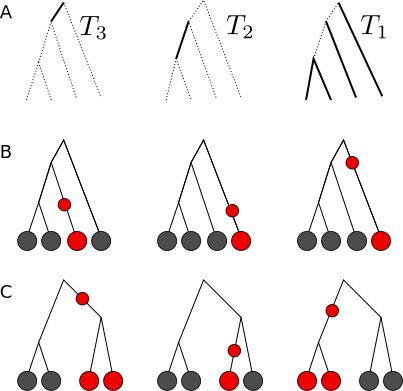
\includegraphics[width=3.5in]{frequency-spectra-trees}
  \end{center}
  \caption{
  \textbf{(A)} The lengths $T_3$, $T_2$, and $T_1$ (see text).
  Note that mutations on $T_3$ are indistinguishable from those on  $T_1$ if the alleles are not polarized.
  \textbf{(B--C)}
  The frequency spectrum encodes information about distributions of tree shape:
  the lower set of trees has longer internal branches, and so will have a higher chance of 2:2 partitions
  than the upper set of trees.
  Mutations (circles on the tree) separate ``red'' from ``black'' types;
  assuming that mutation is independent of the pedigree implies
  that the location of mutation is uniform (proportional to length) on the tree.
  \label{fig:frequency_spectra_trees}
  }
\end{figure}

Suppose we are looking at the empirical distribution of allele frequencies in a sample of size $|A|=n$
at biallelic sites
(the ``allele frequency spectrum'', or ``site frequency spectrum''),
and let $(N_{j,0},N_{j,1})$ denote the numbers of sampled chromosomes that have the '0' and '1' alleles, respectively.
The ``unfolded'' and ``folded'' allele frequency spectra are then
\begin{align}
  a_k^* &= \frac{ \#\{ j : N_{j,0} = k \} }{ |S| } \quad & k &\in \{0,1,\ldots,n\} \\
  a_k &= \frac{ \#\{ j : \min\{N_{j,0},N_{j,1}\} = k \} }{ |S| } \quad & k &\in \{0,1,\ldots,\floor{n/2}\} .
\end{align}
If we have some way of polarizing mutations, so that e.g.\ allele `0' is more likely to be the ancestral allele,
then the unfolded spectrum is more useful;
otherwise, if the choice of allele labeling is arbitrary, 
we expect $a_k^* = a_{n-k}^*$ and the folded spectrum is more natural.

This distribution is obtained by averaging across loci.
Pick a random locus, and call the tree relating the samples at that locus $T$.
Let $|T|$ denote the total length of the tree (in meioses),
and $T_k$ denote the total length of all branches in the tree that are subtended by exactly $k$ tips,
for $1 \le k \le n-1$, so that $|T| = \sum_{k=1}^{n-1} T_k$.
(see figure \ref{fig:frequency_spectra_trees}).
Again assuming that the mutation is independent of inheritance,
the probability that a site has no segregating mutation is
$\exp(-\mu |T|)$, which is the value of $a_0$, up to sampling error.
The probability that only a single segregating mutation has occurred is $\exp(-\mu |T|) \mu |T|$,
and given this,
the location of that mutation is uniform on the tree.
Therefore, the expected contribution of sites with only a single segregating mutation
to $a_k^*$ is $\E\left[ \exp(-\mu |T|) \mu T_k \right]$.
to first order in $\mu |T|$, this says that $a_k^*$ is $\E[T_k]/\E[|T|]$,
the average total number of ancestors of exactly $k$ of the samples
divided by the average total number of ancestors up until the most recent common ancestor of all $n$ samples.



%%%%%%% %%%%%%%%
\subsection{Linkage}

The previous statistics were \emph{single-site} statistics
that took their information from the branching structure of the pedigree
and the differentiating action of mutation along it.
Consideration of the relationships multiple loci brings recombination into the picture.
Perhaps the simplest summary of this is the measure of \emph{linkage disequilibrium}.
It is a two-site statistic, and is in some sense is a single-individual statistic.

Take two sites $j_1$ and $j_2$, at recombination distance $r$,
so that mean number of crossovers that fall between them in a generation is $r$.
Let $I$ be the index of a randomly chosen individual, and $K \in \{m,p\}$,
so that $X_1 = G_{Ij_1K}$ and $X_2 = G_{Ij_2K}$ are the genotypes at $j_1$ and $j_2$ 
on a randomly chosen chromosome, both coded as $\{0,1\}$.
Then the measure of linkage between $j_1$ and $j_2$ is
\begin{align}
  D_{j_1 j_2} = \cov[ X_1, X_2 ] = P_{j_1 j_2}(11) - P_{j_1}(1) P_{j_2}(1) ,
\end{align}
where $P_{j_1 j_2}(11)$ is the empirical frequency of chromosomes that have the `1' allele at both sites $j_1$ and $j_2$,
and $P_{j_1}(1)$ is similar.

\begin{exercise}
  Show that also
  \[ D_{j_1 j_2} = P_{j_1 j_2}(11) P_{j_1 j_2}(00) - P_{j_1 j_2}(10) P_{j_1 j_2}(01) .  \]
\end{exercise}

What does $D_{j_1 j_2}$ have to say about the structure of the ancestral recombination graph?
Intuitively, since it is a correlation between alleles at two loci on the same chromosome,
it should be telling us about how much those loci tend to stick together (and thus have nonindependent).
Fix some number of generations $t$.
Either there has been a recombination between the two loci since that point or there has not;
in the latter case, they are still on the same chromosome.
Let $R_t=0$ if there has been no recombination, and $R_t=1$ otherwise.
By the partition of covariance (\ref{lem:covariance}),
\begin{align}
  \cov[X_1,X_2] &= \cov[ \E[X_1|R_t], \E[X_2|R_t] ] + \E[ \cov[X_1,X_2|R_t] ]  .
\end{align}
Assuming (as usual) that these alleles do not affect the pedigree,
we can see that $\E[X_1|R_t] = \E[X_1]$, and likewise $\E[X_2|R_t] = \E[X_2]$,
since recombinations do not affect the dynamics at single loci.
Therefore, the first term $\cov[ \E[X_1|R_t], \E[X_2|R_t] ]$ is zero.
Now note that $\P\{R_t=0\} = \exp(-tr)$, and so
\begin{align}
  \cov[X_1,X_2] &= e^{-tr} \cov[X_1,X_2|R_t=0] + (1-e^{-tr}) \cov[X_1,X_2|R_t=1] .
\end{align}
Ignore mutation (or take $t$ small enough it contributes little).
Then, we have the covariance of the two alleles as a weighted sum of 
the covariance between two alleles on the same chromosome,
and the covariance between two alleles on different chromosomes,
at a previous time $t$.



This is as far as we can go in general
If we are willing to make the assumption that alleles on different chromosomes


\begin{lemma}{Partition of covariance} \label{lem:covariance}
  For random variables $X$, $Y$, and $Z$, with $\E[X^2]$ and $\E[Y^2]$ finite,
  \begin{itemize}
    \item[(a)]
    \[
      \var[X] = \E[ \var[X|Z] ] + \var[ \E[X|Z] ]
    \]
    \item[(b)]
    \[
      \cov[X,Y] = \E[ \cov[X,Y|Z] ] + \cov[ \E[X|Z], \E[Y|Z] ] .
    \]
  \end{itemize}
  where $\cov[X,Y|Z] := \E[XY|Z] - \E[X|Z]\E[Y|Z]$.
\end{lemma}

\begin{proof}
This follows from the fact that $X,Y \mapsto \E[XY]$ is the inner product on $L^2(\P)$
and the definition of conditional expectation with respect to $Z$ as the orthogonal projection
onto the subspace of $Z$-measurable random variables.
Specifically, $\E[X]$ is the projection of $X$ into the space of constant random variables (since $\E[ (X-\E[X]) c ] = 0$ for any constant $c$);
and $\E[X|Z]-\E[X]$ is the projection of $X$ into the intersection of $Z$-measurable random variables and the orthogonal complement of constant random variables
(since $\E[ f(Z) \E[X|Z] ] = \E[ f(Z) X ]$, by definition of conditional expectation).
Therefore, $X = \E[X] + ( \E[X|Z] - \E[X] ) + ( X - \E[X|Z] )$
is the decomposition of $X$ into three orthogonal subspaces;
and we have a corresponding decomposition for $Y$,
so by Pythagoras,
\begin{align}
  \E[XY] &= \E[X]\E[Y] + \E[ (\E[X|Z] - \E[X])(\E[Y|Z] - \E[Y]) ] + \E[ (X - \E[X|Z])(Y - \E[Y|Z]) ]  \\
  &= \E[X]\E[Y] + \cov[ \E[X|Z], \E[Y|Z] ] + \E[ \cov[X,Y|Z] ] ,
\end{align}
since $\E[\E[X|Z]] = \E[X]$ and likewise for $Y$ and for $XY$.
\end{proof}






%%%%%%% %%%%%%%%
\section{Mate choice: pedigrees}

Now that we have a model for how to produce offspring from two parents,
to model how genes move around in a population,
we need a model for how mates are chosen.
There are various models of ``random mating'',
for instance:

\subsection{The diploid Moran model:}
Continuous-time, fixed population size, overlapping generations.
In continuous time, each individual, at rate 1, chooses another uniformly at random
with whom to mate;
they produce one offspring
that replaces a randomly chosen individual (possibly including the parents).

\subsection{The diploid Cannings model:}
Discrete time, varying population size, nonoverlapping generations.
Suppose at time $t$ there are $N_t$ members of the population,
which we take as a given trajectory.
Each pair of individuals could potentially produce some offspring;
let $X_{ij}$ denote the number produced in this event by pair $(i,j)$ with $i$ as the mother and $j$ as the father for each $1 \le i,j \le N_{t}$.
Suppose that the $X_{ij}$ are \emph{exchangeable},
i.e.\ that $(X_{ij})_{i,j=1}^{N_{t}} \deq (X_{\pi(i)\pi(j)})_{i,j=1}^{N_{t}}$ for any permutation $\pi$ of $(1,2,\ldots,N_{t})$,
and that $\sum_{ij} X_{ij} = N_{t+1}$.
Note that the organisms could be hermaphrodite or unisexual,
as long as we assume that sex determination is independent of siblingship,
and so effectively make sex determination the first step of reproduction.


Each of these produces a \emph{random pedigree}, 
i.e.\ a directed graph with nodes indexed by $(t,k)$, for $1 \le k \le N_t$
and two types of edges, corresponding to maternal versus paternal relationships.
Each arrow represents one meiosis, i.e.\ the result of recombination and segration to produce a gamete.
If we can assume that genetic material does not affect mate choice,
then a model for a population can first choose a random pedigree,
then determine genetic relatedness by making the choices of recombination and segregation
independently in each meiosis.



%%%%%%% %%%%%%%%
\section*{Aside: The genome is not passive}

Of course, the genes an individual carries can have quite a strong influence
on their mate choice, number of offspring, and even on the outcome of recombination and segregation.
In particular, once we know the genomes of every individual, the Cannings model makes no sense,
since individuals are clearly not exchangeable.
This makes things much more complicated,
and we do our best to ignore it,
for instance, by imagining we are tracking only segments of the genome not under selection,
so that genetic variation in fitness only contributes to the distribution of offspring number.



%%%%%%% %%%%%%%%
\section{Allele frequencies: forwards time}

The processes described above keep track of what every individuals' genome is at each point in time.
Now, we need to compute something.
To get our hands on something concrete, consider the marginal process at a single nonrecombining locus.
suppose that there are two possible variants at this locus,
label them `0' and `1',
and denote the frequency of `1's in the population at time $t$ by $P_t$.
Also neglect the influence of mutation.
The change in this frequency is equal to the difference in aggregate numbers offsprings produced by individuals 
carrying each of the two variants,
divided by the population size.
If the locus is neutral
-- i.e.\ an organism's mate choice and offspring numbers are independent of the alleles carried --
then the average number of 

\paragraph{Diploid Moran model:}


%%%%%%% %%%%%%%%
\section{Haploid models}

Take each chromosome as an individual\ldots

\paragraph{The haploid Moran model:}
Continuous-time, fixed population size.
In continuous time, each individual, at rate 1, 
produces one offspring (through simple division)
that replaces a randomly chosen individual (possibly the parent).

\paragraph{The haploid Wright--Fisher model:}
Discrete-time, varying population size.
Suppose at time $t$ there is room for $N_t$ members of the population,
which we take as a given trajectory.
Each individual produces a Poisson number of offspring with large mean;
of the total pool of offspring, a uniformly chosen set of $N_{t+1}$ of these
are chosen to form the next generation.




%%%%%%% %%%%%%%%
\section{Segmenting the genome}

It is possible to compute higher moments -- i.e.\ LD-like statistics across arbitrarily many loci.
For some purposes, it is useful to take a wider view.
Focus for the moment on just two sampled chromosomes.
At any position $x$ along the genome, these two share a common ancestor at some point back in time --
denote the ancestor $A_x$ and the number of generations $\tau_x$.
The entire chromosome, identified with $[0,G)$,
can be then partitioned into the contiguous chunks inherited from distinct ancestors.
More concretely, define $0 = X_0 < X_1 < \cdots < X_{N_R} < L$ as the points along the chromosome 
separating segments that were inherited along distinct paths.
(These could almost be defined as points $x$ such that $A_{x-} \neq A_x$,
but for the possibility of inheriting adjacent segments along more than one path from the same ancestor.)
Define $A_k$ and $\tau_k$ to be the ancestor and coalescent time for the segment $[X_{k-1},X_k)$, for each $1 \le k \le N_R$.
The break points $X$ and associated statistics are essentially unobservable,
but turn out to be very useful anyhow.

Now imagine walking along a chromosome from one end to the other, beginning with the TMRCA $\tau_0$ at the end of the chromosome.
As is made formal below,
the distance we have to go before $X_1$ is Exponential with rate $\tau_0$,
and $R_1$, the time back to the recombination that switched us from one path through the pedigree to another is uniform on $[0,\tau_0]$.
% NOTE not quite right since it could fall on either path back to the ancestor which could be different lengths
The distribution of $\tau_1$ depends on $\tau_0$ and on $R_1$ but not on $X_1$.
Similarly, the $X_2-X_1$ and $R_2$ are conditionally independent of each other and everything else so far given $\tau_1$,
but then $\tau_2$ depends on $\tau_0$, $\tau_1$, $R_1$, and $R_2$.
The entire sequence along a chromosome of length $G$ can be generated
by first sampling an infinite sequence $\tau_0,\tau_1,\tau_2,\ldots$,
then sampling $L_1', L_2', \ldots$ to be independent Exponentials with $\E[L_k] = 1/\tau_k$,
defining $N = \min \{n : \sum_{k =1}^n L_k' \ge G \}$,
then letting $L_k = L_k'$ for $1 \le k < N$ and $L_N = G - \sum_{k =1}^N L_k'$.
The sequence $\tau$ is stationary
and with the property that $(\tau_1, \tau_2, \ldots, \tau_n) \deq  (\tau_n, \tau_{n-1}, \ldots, \tau_1)$ for each $n$.


\begin{figure}[ht!]
  \begin{center}
    \includegraphics[width=\textwidth]{IBD-sequence-diagram}
  \end{center}
  \caption{
  Sequnce of coalescent times $\tau$, recombination times $R$, and IBD lengths $L$ along a chromosome.
  }
\end{figure}

\begin{lemma}{Joint distribution of neighboring shared segments}
  \begin{enumerate}
      
    \item[(a)] Conditioned on $X_{k-1}$ and $\tau_{k}$, the length $X_k-X_{k-1}$ has the same distribution as $\max\{Z/\tau_k,G-X_{k-1}\}$,
      where $Z$ is an independent Exponential random variable with mean 1,
      and the time $R_k$ has a uniform distribution on $[0,\tau_k]$, independent of $X_k-X_{k-1}$.

    \item[(b)] Let $(X_-,R_-)$ and $(X_+,R_+)$ be the locations and recombination times of the closest events
      to the left and right of $x$, respectively.
      Let $Z_-$ and $Z_+$ be independent Exponential random variables with mean 1.
      Conditioned on $\tau_x$, all four are jointly independent,
      with $X_- \deq \max\{ x-Z_-, 0 \}$ and $X_- \deq \min\{ x+Z_+, G \}$;
      and $R_-$ and $R_+$ uniform on $[0,\tau_x]$.

  \end{enumerate}
\end{lemma}

\begin{proof}

  \textbf{(b)} The probability that there were no crossovers in the segment $[x,x+y)$ in any of the $2\tau_x$ meioses on the path back to $A_x$
  is, by definition, $\exp(-x \tau_x)$ -- and hence, the distance along the chromosome to the next recombination event that causes a switch is exponential with rate $\tau_x$,
  and the first such recombination event is uniformly distributed across the possible meioses,
  by properties of competing Poisson processes.

  Part (a) follows from (b) by conditioning on $X_- = x$.

\end{proof}

\begin{lemma}{The sequence of coalescent times determines the distribution of IBD lengths.}
  Conditioned on $(\tau_1, \ldots, \tau_{N_R})$, 
\end{lemma}


